
\subsection{Code Deployment \& Image Building}
\begin{figure}[H]
    \centering
    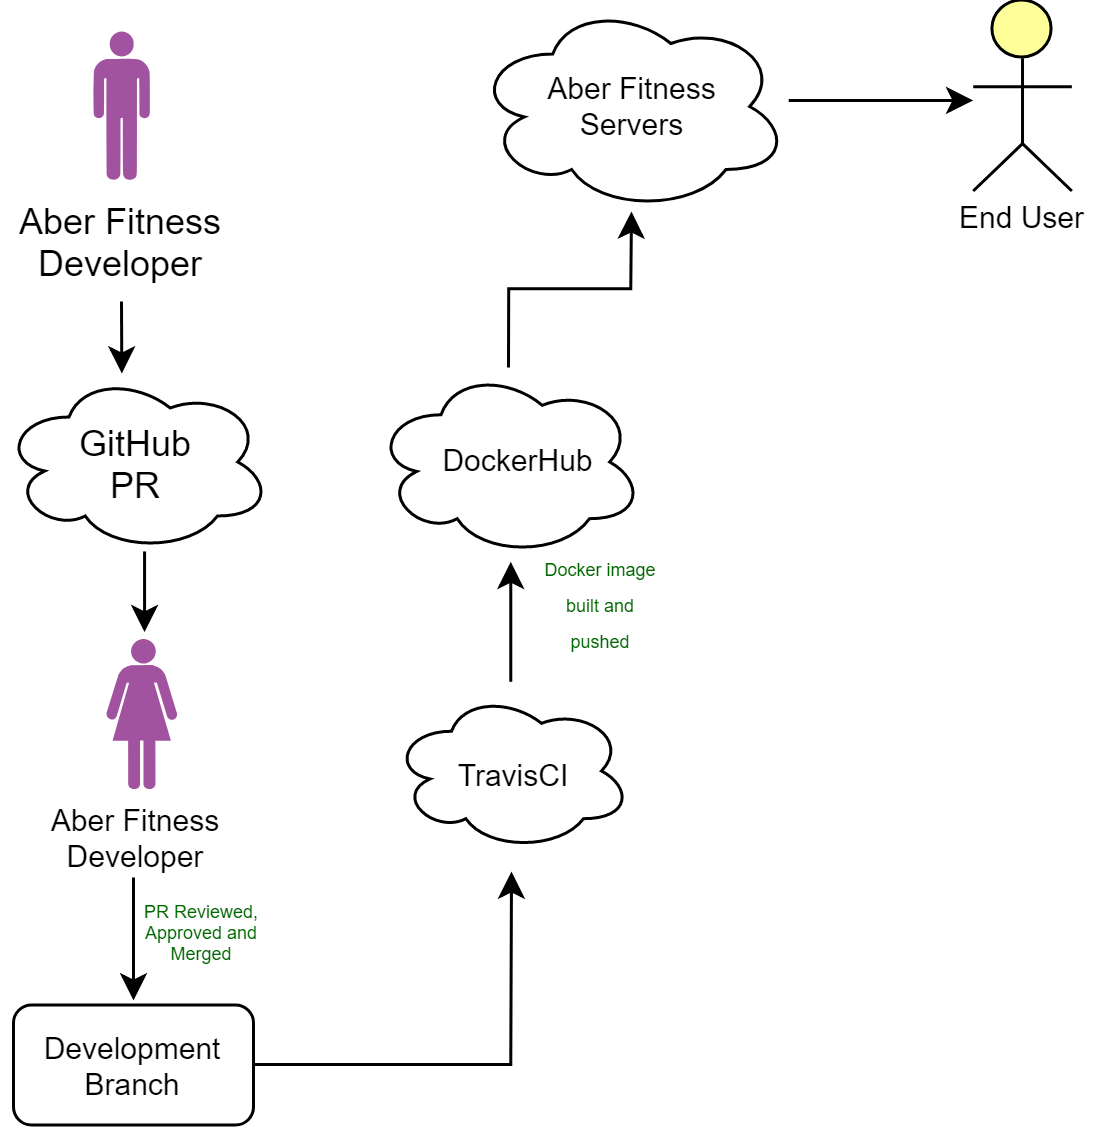
\includegraphics[width=0.7\textwidth]{Images/diagram_af.png}
    \caption{Aber Fitness development process flow diagram}
    \label{fig:development_flow_diagram}
\end{figure}

The development flow diagram (Fig. \ref{fig:development_flow_diagram}) outlines the deployment and code review process. Following the pull request being reviewed by another member of the team and Travis CI building the application to ensure that all unit tests passed, the pull request would then be merged into the \lstinline{development} branch. Any pushes to the \lstinline{development} branch would trigger Travis CI to then run a script within the application repository, \lstinline{bin/docker.sh}. This script was responsible for building the application into a Docker image and pushing it to Docker Hub. Once the image had been built and pushed, the application would then be ready for deployment to the staging host, \textit{docker2.aberfitness.biz}. The developer could then issue the \lstinline{/deploy} command within Slack to begin the re-deployment of the entire Docker stack\footnote{A 'stack' is a collection of Docker images grouped together through a \textbf{docker-compose.yml} file}. The command triggered a webhook to automatically run the commands necessary to deploy the new images to the stack. 

This deployment flow proved quite effective throughout the development process, allowing code updates to easily be deployed to \textit{docker2.aberfitness.biz} while ensuring that code had been peer reviewed and unit tested before being rolled out onto a live server. The deployment flow relied heavily upon GitHub and Travis, as they were responsible for hosting the code and generating Docker images respectively. While the majority of the time these services worked out notably well, there were a few issues during incidents where Travis CI was suffering from outages; the implications of these outages were that deployment of code updates was made impossible \textemdash adding some delays to the development process.


